\documentclass[11pt]{article}
\usepackage[margin=1in]{geometry}          
\usepackage{graphicx}
\usepackage{amsthm, amsmath, amssymb}
\usepackage{setspace}\onehalfspacing
\usepackage[loose,nice]{units} %replace "nice" by "ugly" for units in upright fractions
 \usepackage[UTF8, heading = false, scheme = plain]{ctex}
 \usepackage{hyperref}
 \usepackage{color}
\usepackage[normalem]{ulem}
\usepackage{url}
\usepackage[dvipsnames]{xcolor}


\DeclareUrlCommand\ULurl{%
  \renewcommand\UrlFont{\ttfamily\color{blue}}%
  \renewcommand\UrlLeft{\uline\bgroup}%
  \renewcommand\UrlRight{\egroup}}
 
\title{两种阅读理解模型框架的概要介绍}
\author{徐俊}
\date{2016年12月}


 
\begin{document}
\maketitle

\section{摘要}
让机器具备阅读理解能力是自然语言研究者长久以来追求的核心目标之一,随着深度学习技术的兴起和阅读理解相关大数据集的发布,二者结合引爆了当前人们对于阅读理解研究的兴趣。本文概要介绍阅读理解任务和当前两种“经典”神经网络模型,同时给出模型的开源代码和实验所需数据集,便于读者快速上手。

\section{阅读理解任务简介}
作为自然语言处理方向乃至人工智能领域的一个核心任务,让机器具备阅读理解能力的研究受到人们广泛而持续的关注。

为了考察人类的阅读理解能力,往往采取提问的方式,即:给定一篇文本和与文本相关的问题,要求给出该问题的答案。同样的方式也被用于衡量机器的阅读理解能力,在谷歌公司Hermann(Hermann et al. 2015)\cite{hermann2015teaching}发布的CNN数据集中,数据以三元组的形式存在:文本、问题和答案,机器阅读文本和问题然后给出答案。

CNN数据集,是基于美国有线电话新闻网(The Cable News Network)的新闻构建的,其中新闻内容会作为“文本”,而“问题”则是新闻的标题(扣除其中一个实体,使用@placeholder标记),“答案”是被抠除的那个实体。文本中的实体(人名、地名、机构等)均被替换成标记符(@entity),同一个实体使用同一个标记符表示,答案是一个在文中出现的实体,其在问句中的位置用特殊标记@placeholder表示。Figure~\ref{fig:1} 展示了CNN数据集中的一个三元组。

\begin{figure}[htbp]
\begin{center}
	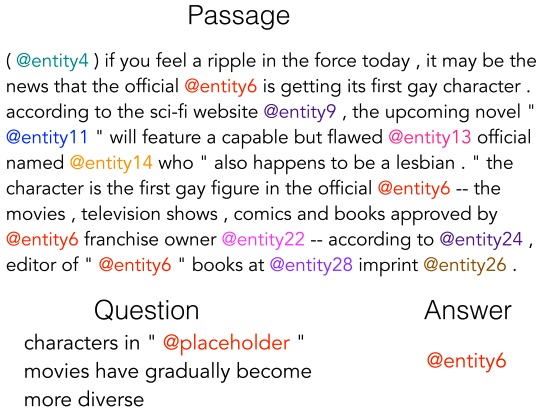
\includegraphics[width=80mm]{picture/CNN.jpg}
	\caption{CNN数据集的一个样例\cite{chen2016thorough}。}
	\label{fig:1}
\end{center}
\end{figure}

需要注意的是,在CNN数据集中答案是一个出现在文本中的一个词(实体),而其他数据集却不一定如此,比如在斯坦福大学Rajpukar\&Liang发布的SQuAD\cite{rajpurkar2016squad}数据集中的答案就可能是由多个词组成且不一定是实体。本文的阐述基于CNN数据集。

\section{模型}
随着深度学习技术的再度兴起,神经网络模型成为阅读理解任务中的主流模型。下面简要的介绍其中两种具有代表性的模型。
\subsection{Attention Reader}
Attention Reader\cite{hermann2015teaching}在处理的时候,首先采用双向RNN分别表示文本(看做一个“长句子”)和问句,再利用attention机制寻找文本表示中同问句相关的信息,最后根据相关程度提取文本信息做分类并给出预测的答案。Figure~\ref{fig:2}是Attention Reader的模型框架图。

\begin{figure}[htbp]
\centering
\begin{minipage}[t]{0.45\textwidth}
\centering
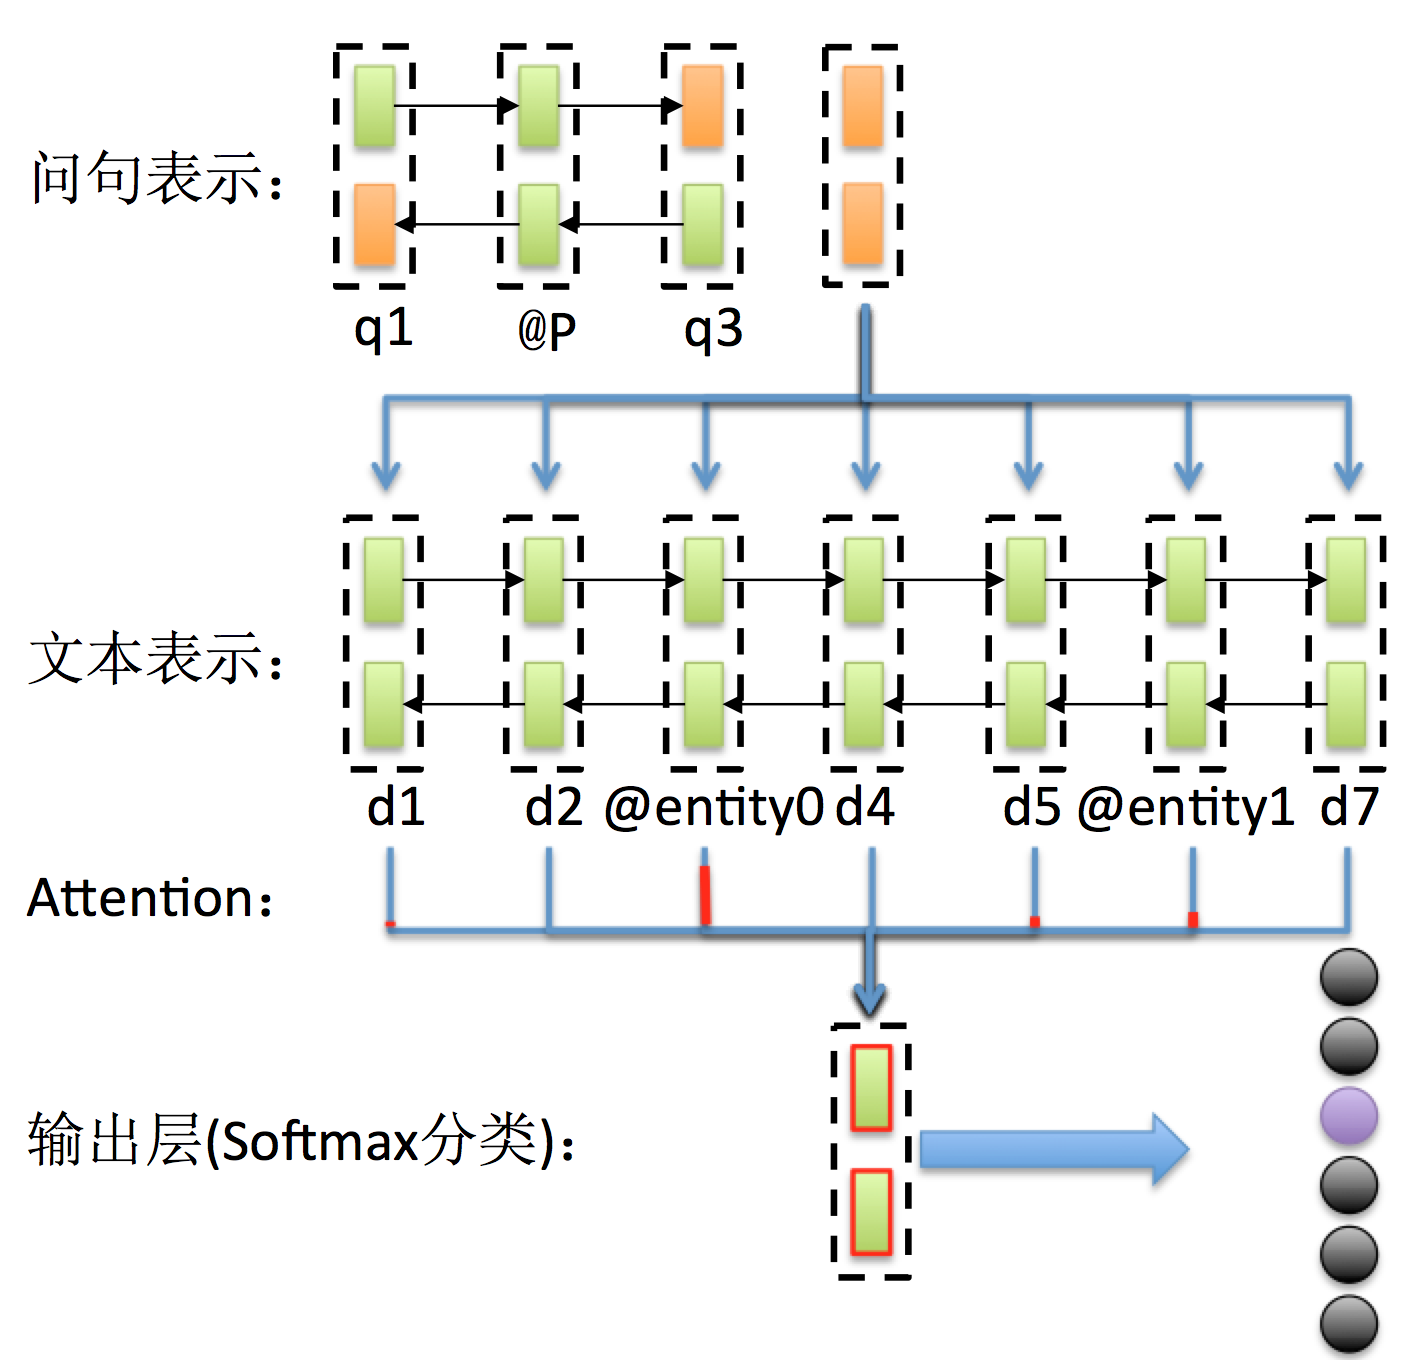
\includegraphics[width=70mm]{picture/attentionreader.png}
\caption{Attention Reader}
\label{fig:2}
\end{minipage}
\begin{minipage}[t]{0.45\textwidth}
\centering
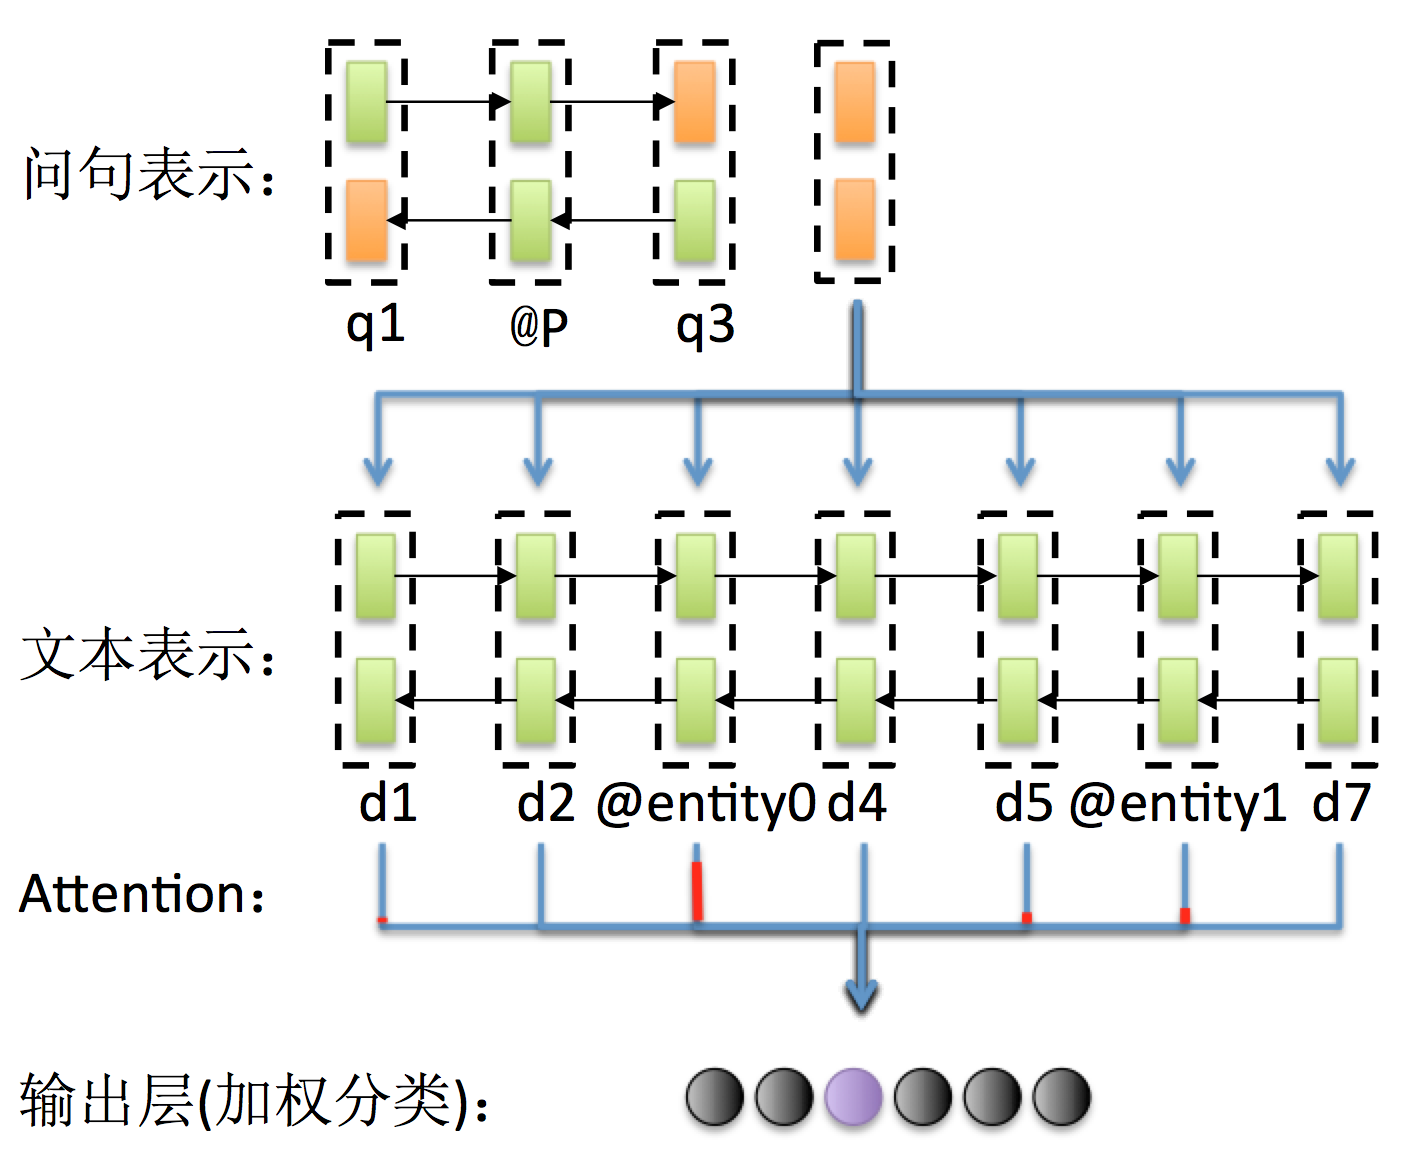
\includegraphics[width=70mm]{picture/attensumreader.png}
\caption{Attention-Sum Reader}
\label{fig:3}
\end{minipage}
\end{figure}

\begin{enumerate}
    \item {\bf 表示}:使用双向RNN(LSTM Cell)获取文本表示和问句表示。其中问句表示分别由双向RNN两个方向各自最后一个时刻的隐层状态(图中左上角双向RNN中的橙色向量)拼接而来;
    \item  {\bf Attention}: 使用Attention机制获得文本中各个时刻的隐藏状态向量同问句表示之间的相关程度(也就是权重,最简单的做法就是向量点乘),在图中用红色线条表示(越长表示相关程度越高);
    \item  {\bf  输出层}:文本各个时刻隐藏状态向量乘以对应时刻的权值,加和,获取“提取后的文本信息”,过softmax在词表上进行分类;
\end{enumerate}
%\begin{figure}[htbp]
%\begin{center}
%	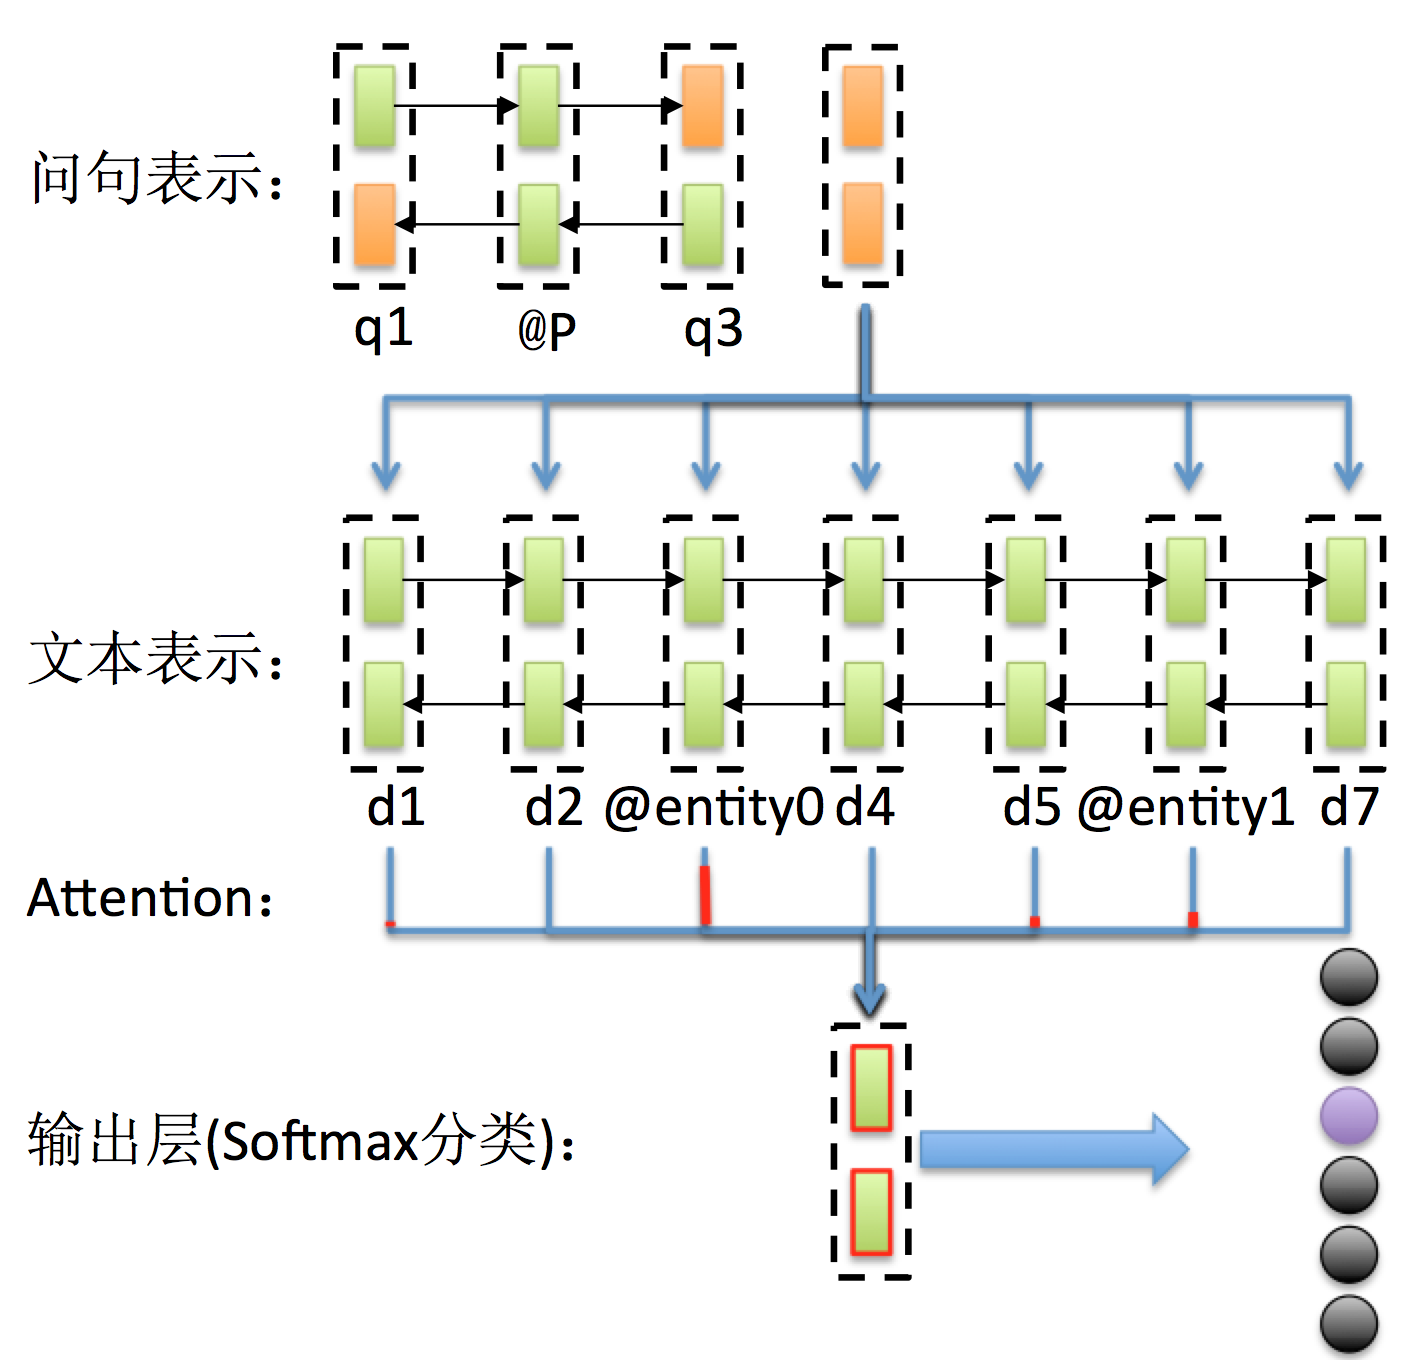
\includegraphics[width=80mm]{picture/attentionreader.png}
%	\caption{Attention Reader}
%	\label{fig:2}
%\end{center}
%\end{figure}

在Attention Reader中,核心的思路是通过动态的attention机制从文本中“寻找相关信息”,再做依据该信息给出预测结果。关于该模型的具体实现有多个不同的版本,斯坦福大学的Chen\&Manning(Chen et al. 2016)\cite{chen2016thorough}利用该模型在CNN测试集上取得了72.4\%的效果(当时最好效果),Chen在ACL2016会议中报告该模型的最新效果为73.8\%。

\subsection{Attention-Sum Reader}
IBM公司的Kadlec(Rudolf Kadlec et al. 2016)\cite{kadlec2016text} 提出了Attention-Sum Reader,该模型直接利用attention机制基于问句表示在文章中寻找最相关的词作为答案。

Figure~\ref{fig:3}是Attention-Sum Reader的框架图,可以直观看出Attention-Sum Reader同Attention Reader在模型框架上几乎类似。
%\begin{figure}[htbp]
%\begin{center}
%	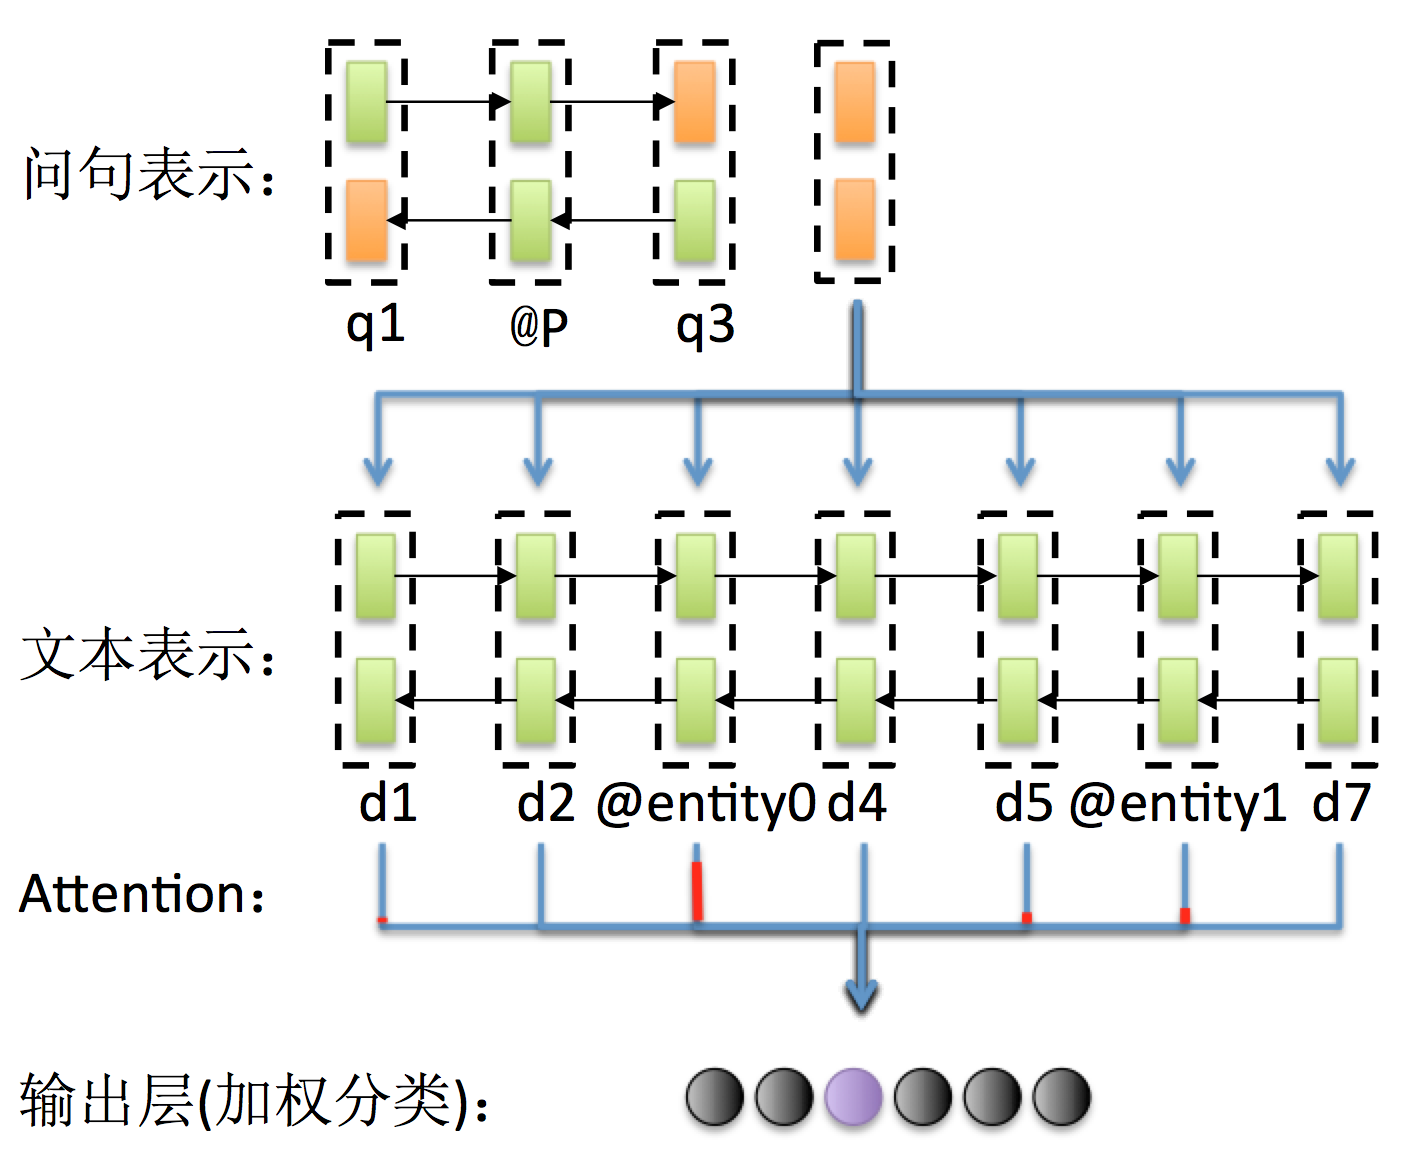
\includegraphics[width=80mm]{picture/attensumreader.png}
%	\caption{Attention-Sum Reader}
%	\label{fig:3}
%\end{center}
%\end{figure}
Attention-Sum Reader直接利用attention机制获取文本中各个位置作为答案的概率\textcolor{gray}{(需要将同一词语在文本中不同位置的概率加和作为该词语成为答案概率)},而不再同Attention Reader最后一步那样,通过分类(softmax)获取各个词语作为答案的概率。

虽然做法上同Attention Reader区别不是特别明显,但是这是两种不同的思路,基于此而衍生出来的模型的变种则差别甚大。{\bf 二者的本质区别在于最终提供给输出层的信息(特征)类型,Attention Reader输入给输出层的是经过attention机制加权后的文本表示,也就是“根据问句在文本中提取的信息”,而Attention-Sum Reader输入给输出层的是attention结果本身。}

\subsection{对比}
(Rudolf Kadlec et al. 2016)\cite{kadlec2016text} 报出的效果是69.5\%,但是在我们的实现中获得了73\%的效果。可见,{\bf 两个Reader本身的性能在伯仲之间}。

Attention Reader的输出层为词表中每个词学习一个权重向量,而其中有效候选词是真实实体的指代(如@entity0),指代在不同的文本中代表不同的真实实体,这就使得有效候选词的权重向量在一定程度上并不能刻画这个词,进而加大学习难度。而Attention-Sum Reader中这个问题则要小的多,其直接利用问句表示在文本中寻找最相关的词。

Attention-Sum Reader的问题在于其严重依赖于问句表示,Attention Reader在“文本中寻找相关信息”是对于问句表示的丰富,毕竟,目标词的表示并不等同于问句表示。

\section{数据集和开源代码}

\subsection{开源代码}
Attention Reader\cite{chen2016thorough}(Theano): \ULurl{https://github.com/danqi/rc-cnn-dailymail};

 \noindent Attention-Sum Reader\cite{kadlec2016text}(Theano): \ULurl{https://github.com/rkadlec/asreader};

\subsection{数据集}

CNN\&Daily Mail dataset: \ULurl{http://cs.nyu.edu/~kcho/DMQA/};

 \noindent More datasets for QA: \ULurl{https://github.com/karthikncode/nlp-datasets};
 
 \section{总结}
本文概要的介绍了阅读理解任务,以及两种“经典”的阅读理解模型,同时给出对应开源代码和相关数据集,方便对该领域有兴趣的读者快速上手,实践出真知。
 
\bibliographystyle{plain}
\bibliography{acl}
\end{document}
